% !TeX spellcheck = en_US
\documentclass[]{TAACpaper}
\usepackage[linesnumbered,boxed]{algorithm2e}
\pagestyle{plain}
\begin{document}

%This is the comment. Further under the text features of use of style of theses are described

%We are specifying language of the paper
\selectlanguage{english}
\def\dd#1#2{\frac{\partial#1}{\partial#2}}
\section{
%%%%%%%%%%%%%%% You have to specify name of your paper here
``Investigation of tuning parameters of Tabu Search algorithm and its modification  for solving the Routing Courier Delivery Problem.''
}

\authors{
R.~Shafeyev , L.~Lyubchik 
}

\abstract{
%%%%%%%%%%%%%%% You have to insert abstract of your paper here

The paper considers the Routing Courier Delivery Problem with the service time for which the discrete model was constructed and the calculation scheme based on the Tabu search algorithm. This article provides a method for dynamically adjusting the parameters of Tabu Search algorithm in the process of solving the problem. The efficiency  of the proposed algorithm‘s scheme has been tested on large-scale problems, which were generated on the basis of well known model routing problems.

}

%%%%%%%%%%%%%%% To define new section use a command \subsection
% We are defining "Introduction" here
\subsection{Introduction}
One means of saving resources for transportation of goods is the use of decision support systems in the field of transport logistics. One of the key functions of decision support systems in the field of transport logistics is the ability to calculate and construct efficient detour routes for various purposes in the transport network in terms of cost. The mathematical formulation of this problem is widely known as the Vehicle Routing Problem (VRP). There are several types of VRPs with various additional conditions such as the carrying vehicle`s capacity, time of deliveries and other limitations for a better description of the environment.

This article is devoted to the courier routing problem, which is a sub-problem of VRP. The problem is to find a route to visit a given set of addresses by a number of units of vehicles carrying goods from the sender to the recipient.

Automation of the route planning process will be relevant for: online stores, large wholesale companies (e.g. for distribution of goods that are perishable or optimizing the delivery schemes of goods to destinations) and firms with the aim of organizing restocking in stores. A practical application of the problem can be found in the transportation of patients between the buildings of clinic \cite{Beaudry, Kergosien}, the delivery of newspapers and magazines and the delivery of fuel to homes \cite{Sarak}. The solution of these problems also has a practical application in the helicopter transportation system of people between offshore oil platforms \cite{Romero}.

In recent years are an increasing amount of people turning to courier services for famous needs.Typically, client orders placed the day before and the dispatcher then has a full list of orders that must be delivered within the deedlines started by the client. Attanasio \cite{Attanasio} held a thematic research on courier services which described the advantages of using computer technologies to human dispatching. In his work he considered examples of work by eCourier Ltd, a London company that offers express services. Their clients are mainly law firms, financial institutions, advertising agencies and other organizations that are interested in the rapid delivery of goods or the sensitive documents. Once all of the orders at a particular time have been placed, you must create a route that would satisfy the requirements of the customers. Depending on the service level that was specified by the client, the courier can combine several products customers.

Companies that offer courier services frequently have a mixed fleet of vehicles, which consists of bicycles, motorcycles, cars and small trucks. Depending on the type of request, the transport arrangement means and time slots will be selected the kind of vehicle that will be able to execute the order within a specified time. Researches \cite{Attanasio} showed that the using of computer methods, including optimization algorithms have been very profitable for courier companies.

Thus, the use of an automated system allows to improve the quality of service, reduce delivery time, improve courier efficiency and reduce the cost of shipping, thereby providing a competitive advantage increase.

\subsection{Problem Statement}
Let $C,dim(C)=n$ be a set of vehicles and $Q,dim(Q)=m$ be a set of requests received from customers at the current time.

Suppose that the following information is known about vehicles from set $C$: \\
$\vec{P}_c$ -- vehicle position, $c \in C$;\\
$L_c$ -- vehicle capacity, $c \in C$.

Let $S$ be a set of senders, ($dim(S) = dim(Q) = m$), $R$ is a set of receivers, $dim(R) = dim(Q) = m$. Then each client request $q \in Q$ includes the following information:\\
$s_q$ -- a sender of client shipment, $s \in S$; \\
$r_q$ -- a receiver of client shipment, $r \in R$; \\
$\vec{P}_{s_q}$ -- sender position;\\
$\vec{P}_{r_q}$ -- receiver position; \\
$w_q$ -- client shipment that is required to be delivered from the sender to the recipient; \\
$[t_{s}^{q}, t_{s}^{q}+ \Delta{t_{s}^{q}}]$ -- the time window within which the worker must to pick up the goods from the sender;\\ 
$[t_{r}^{q}, t_{r}^{q}+ \Delta{t_{r}^{q}}]$ -- the time window within which the worker must deliver the goods to the receiver.
 
Thus, each request can be represented as a tuple:
\begin{equation}
\forall q \in Q: q = (s_q,r_q, \vec{P}_{s_q}, \vec{P}_{r_q}, w_q, t_{s}^{q}, \Delta{t_{s}^{q}}, t_{r}^{q}, \Delta{t_{r}^{q}})
\end{equation}
To estimate the cost of transportation between destinations defined by the following cost function $\Omega$:
\begin{equation}
\forall i,j \in S \cup R: \exists \Omega_{i,j} = \Omega(\vec{P}_i,\vec{P}_j)
\end{equation}

It is necessary to construct the most optimal routes of vehicles movement for the transportation of goods from the sender to the receiver for all client requests.

\begin{figure}[h]
	\hfil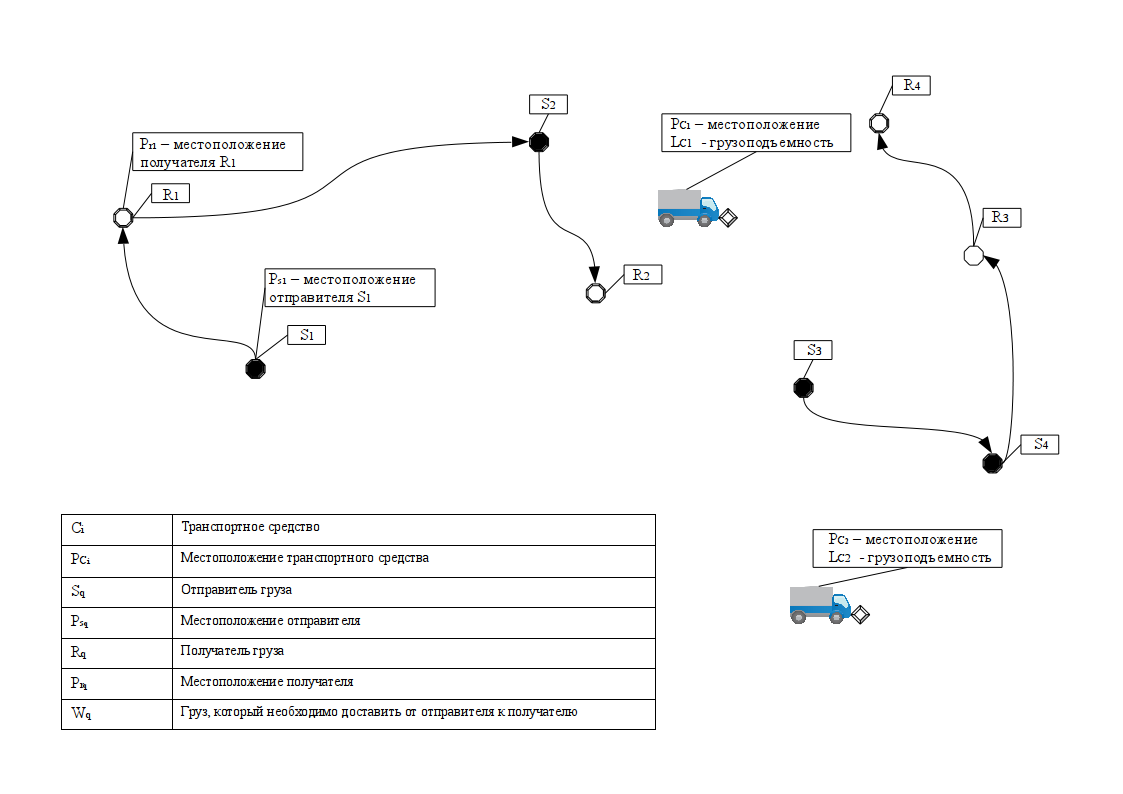
\includegraphics[height=4.0in]{images/scheme}\hfil
	\caption
	{
		Example of the Routing Delivery Problem.
	}
	\label{aba:fig1}
\end{figure}

\subsection{Discrete model}
The Routing Courier Delivery Problem can be represented as a directed graph $G=G(V,E)$. The set $V=C\cup{S}\cup{R}$ are nodes of the graph $G$, with elements consists of vehicles, senders and receivers. $E$ -- dynamic set of arcs of the graph $G$, such that:
\begin{equation}
\forall e(X) \in E: e(X) = (v_i,v_j), \exists v_i \in V, v_j \in V/C
\end{equation}

Let $X = \{X^k\}^n_{k=1}$ is a sequence of variable matrices for each vehicle $k \in C$. Elements of the matrices take the following values:
\begin{equation}
  x^{(k)}_{i,j} = 
    \begin{cases}
	  1,&\text{the vehicle $k \in C$ moves from the $i$ node to the $j$}\\
	  0,&\text{otherwise.}
    \end{cases}
\end{equation}
where: $i\in{V/C \cup {k}}, j \in V/C$.

Let us introduce the vector  of variables $ \vec{Y}  ^ k(X) $ for each vehicle $ k \ in C $. Vector elements have the following values:
\begin{equation}
\vec{y}^{(k)}_{j}(X) = 
\begin{cases}
1,&\text{the request $j \in Q$ is processed by vehicle $k \in C$}\\
0,&\text{otherwise.}
\end{cases}
\end{equation}
where: $i\in{V/C \cup {k}}, j \in V/C$.


Let $t^k_j(X^{(k)})$ -- arrival time of the vehicle $k \in C$ at the destination $j \in S \cup R$. 

The objective function takes the following form:
\begin{equation} \label{main_objective}
  F(X) = 
    \sum_{k \in C}
     \sum_{i,j\cup{V}} 
     \Omega_{ij} \cdot x_{ij}^{(k)} 
     \to min
\end{equation}

We define constraints on the objective function (\ref{main_objective}), which provided the continuity of routes:
\begin{align} 
& \sum_{k \in C}\sum_{j \in S \cup R}x^{(k)}_{i,j} \leq 1, 
\forall i \in V \label{main_cond_1}\\
& \sum_{k \in C}\sum_{i \in S \cup R \cup \{k\} } x^{(k)}_{i,j} = 1, 
\forall j \in S \cup R \label{main_cond_2}\\
& \sum_{i \in S \cup R \cup \{k\} } x^{(k)}_{i,\omega} - 
\sum_{j \in S \cup R} x^{(k)}_{\omega,j} \leq 1, 
\forall \omega \in S \cup R,  \forall k \in C \label{main_cond_3}\\
&  \sum_{i \in S \cup R / Z}\sum_{j \in Z } x^{(k)}_{i,j} > 0, 
Z=\{z \in Z: \sum_{j \in S \cup R}x^{(k)}_{j,z}>0 \}  ,\forall k \in C \label{main_cond_4}
\end{align}

The restriction (\ref{main_cond_1}) prohibits a node in the graph $G$ of having more than one output arc. The restriction (\ref{main_cond_2}) prohibits a node from having more than one input arc.  The constraint (\ref{main_cond_3}) indicates that the number of input arcs to the node can not be less than the output arcs (this constraint considers the fact that the vehicle can leave the destination only if it has visited this node). The restriction (\ref{main_cond_4}) excludes local loops.

The next constraints synchronize values of variables $X$ and $\vec{y}$ for each request $q \in Q$ and prohibits the courier service visiting the receiver before meeting with the sender first:
\begin{align} 
& x^{(k)}_{s_q} + x^{(k)}_{r_q} = 2 \cdot y^{(k)}_{q}(X), \forall k \in C, q \in Q  \\
& y^{(k)}_{q}(X) \cdot (\tilde{t}^k_{r_q}(X^{(k)})-\tilde{t}^k_{s_q}(X^{(k)})\ge{0}, \forall k \in C, q \in Q
\end{align}

Defining restrictions for the accounting of vehicle capacity and delivery time windows:
\begin{align} 
& \sum_{j\in{Q}} \omega_j \cdot y_{j}^{k} \leq L_k, \forall{k}\in{C}\\
& t_{s}^{q} \leq \tilde{t}^k_{s_q}(X^{(k)} \leq t_{s}^{q}+ \Delta{t_{s}^{q}}, \forall q \in Q, \label{tws_cond} \\
& t_{r}^{q} \leq \tilde{t}^k_{r_q}(X^{(k)} \leq t_{r}^{q}+ \Delta{t_{r}^{q}}, \forall q \in Q, \label{twr_cond}
\end{align}



\subsection{Description of the Algorithm}
We present the set of matrices $\{X^k\}$ in the form of a vector defined on the hypercube $E^\eta=\{0.1\}^\eta$, where $\eta=n\cdot(2m+1)\cdot 2m$. The aim of the task is to minimize the objective function:
\begin{align} 
& F(\vec{u})\to min,\vec{u}\in E^{\eta}
\end{align}	

Denote by $\delta(\vec{u},\vec{v})$ the Hamming distance between $\vec{u}$ and $\vec{v}$. Through $N_l(\vec{u})$ we denote the neighborhood of a point $\vec{u}$ radius $l$\cite{vrp_shafeyev}:
\begin{align} 
& N_l(\vec{u})=\{\vec{v} \in E^{\eta}:\delta(\vec{u},\vec{v})\le l \}, l=\bar{1,\eta}
\end{align}	

When $l=\eta$ a set $ N_l(\vec{u})$ for any vector $\vec{u}$ coincides with the set $E^{\eta}$ and being in this neighborhood vector with a minimum value of the objective function is equivalent to solving the original problem. The classic Local Search algorithm starts with a randomly selected vector $\vec{u^0}$.
On the $i$ step of the algorithm the current vector moves to the minimum value of the objective function in the neighborhood:
\begin{align} 
& F(\vec{u}^{i+1})=min\{F(\vec{v}):\vec{v} \in N_l(\vec{u}^i)\}
\end{align}	

The algorithm terminates at a local optimum, when $F(\vec{u^{i+1}})=F(\vec{u^i})$. In VRPs there are a typical situation when many local optimums and only one of them is global:
\begin{align} 
& F_{opt}=min\{F(\vec{v}):v \in E^{\eta}\}
\end{align}	

To ensure that the algorithm does not stop at a local minimum and move from one local optimum to another, we must remove the central point  from the current neighborhood and when the algorithm searches for the minimum, the following rule applies. Let $l=2$ and the current position moves from $\vec{u^{i}}$ to $\vec{u^{i+1}}$ therefore changing the values in the coordinate $(u_\lambda^{i}, u_\omega^{i})$. The algorithm stores such pairs for the last $h$ amount of steps and in the next step prohibits the movement in these directions. An ordered list of such pairs:
\begin{align} 
& \phi^i=\{(u_\lambda^{i},u_\omega^{i}),(u_\lambda^{i-1},u_\omega^{i-1}),\cdots,(u_\lambda^{i-h+1},u_\omega^{i-h+1}) \} 
\end{align}	
is called the Tabu List. The pair $(u_\lambda,u_\omega),\lambda \ne \omega$ does not prohibit the movement of pairs $(u_\lambda,u_\lambda)$ and $(u_\omega,u_\omega)$. When $l > 2$, the Tabu List is created accordingly for 3 coordinates, 4 coordinates, etc. A set of non-restricted vectors are denoted by $N_l(\vec{u^i},\vec{\phi^i})$. In order for the search to be efficient, it is advisable to use small values of $h$ and to control this parameter throughout the algorithm.

\begin{algorithm}[H]
	\textbf{function TabuSearch}($u^0,l,p,h$) \\
	// Initial variables:	\\
	$u^{opt} = u^0$
	$F^{opt} = F^0$
	$\phi^{0} =  \emptyset$
	$i=0$ \\
	\While{the breakpoint is not triggered }{
	   $N_l = N_l(u^i,\phi^i,p,h) $ \\
		\eIf{$N_l \ne   \emptyset $}{
			$ u^{i+1} = u^i$ \\
			$i = i + 1$ \\
			\textbf{goto} 5
		}
		{
			// find optimum into the neighborhood $N_l$: \\
			$ u^{i+1} : F(u^{i+1}) = min\{ F(y): y \in N_l \}$
		} 

		\If{$F(u^{i+1}) < F_{opt})$}{
			$ F_{opt} = F(u^{i+1})$ \\
			$ u^{opt} = u^{i+1}$
		}
			
		
		$\phi^{i+1} = update(\phi^i)$\\
		i = i + 1\\
	   
	}
	\textbf{return} $u^{opt}$
	
\caption{Pseudo-code for probabilistic Tabu Search algorithm.}
\label{alg:TabuSearch}
\end{algorithm}

Denoted by $N_l(\vec{u^i},\vec{\phi^i},p)$ a probabilistic neighborhood which stems from a deterministic $N_l(\vec{u^i},\vec{\phi^i})$ as follows; each vector $\vec{v} \in N_l(\vec{u^i},\vec{\phi^i})$ with probability $p$ is included in the neighborhood $N_l(\vec{u^i},\vec{\phi^i},p)$ regardless of other points. Note that this set may be empty or contain only one point. The General scheme of the probabilistic Tabu Search algorithm in scheme \ref{alg:TabuSearch} is referred to as the pseudo-code.

The stopping criterion is based on the total number of steps $N_{stop}$, which does not change the value $F_{opt}$. Values $l,p,h$ are the control parameters of the algorithm. Their choice depends on the problems dimension.

In the presented scheme, it was assumed that the value of $h$ (the dimension of the Tabu List) does not change throughout the course of the algorithm. This creates certain difficulties in the implementation of the scheme, as it is unknown how long the Tabu List size should be. At small $h$ the algorithm can get into an infinite loop. At large $h$ the search becomes inefficient.


\subsection{Initialization}
To use the Tabu Search Algorithm, you must first build the initial solution. For the initial solution $ \vec{u^0} $, you can use the heuristic method of route constructing\cite {Cordeau2001, Braysy}. The essence of these methods is as follows. According to the rules of the algorithm routes for each vehicle are constructed as client requests come in order to ensure efficiency.  
To preserve the order of visits of the nodes by the vehicles in the pair are ordered ''sender-receiver''.This algorithm is fast enough (computational complexity $O(n^3)$ \cite{Babb}), so it is convenient to use for the initialization of the vector $\vec{u^0}$.

At the beginning of the algorithm a single request is added to each route in accordance with the time constraints. The first node(sender) is chosen randomly or is selected the one you want to perform before others. Then every possible request $u$ from the set of unchecked requests $ Q' $ (the set $ Q'\in Q$) is estimated by inserting it in the beginning of the route, or the end of the route between two adjacent nodes. the following criteria is used to select the insertion point:
\begin{align} 
\label{insert_kr}
c(k,v_i,u,v_{i+1}) = \min =
\begin{cases}
\min_{q=2,\dots,n^k}(\Omega_{q-1,u}^k+\Omega_{u}^{k}+\Omega_{u,q}^{k}-\mu \Omega_{q-1,q}^k),\\
\Omega_{k,u}^k+\Omega_{u,q}^k+\Omega_{u}^k\mu \Omega_{q,q}^k), q=1\\
\Omega_{q,u}^k+\Omega_{u}^k, q=n^k
\end{cases}
\end{align} 
where:\\
$k$ --  a vehicle route $k\in C$;\\
$n^k$ - a number of nodes in the route;\\
$\mu$ --a tuning parameter, $\mu \ge 0 $;\\
$\Omega_{u}^k=\Omega^k[\vec{P}_{s_q}, \vec{P}_{r_u}]$ -- insert a new request between existing sender and receiver;\\
$\Omega_{u,q}^k=\Omega^k[\vec{P}_{r_u}, \vec{P}_{q}]$ -- insert a new request between existing sender and receiver to the begining of the route;\\
$\Omega_{q,u}^k=\Omega^k[\vec{P}_{q}, \vec{P}_{s_u}]$ -- insert a new request between existing sender and receiver to the end of the route.

Adds that request, which $c(k,v_i,u,v_{i+1})$ will be minimal:
\begin{align} 
\label{kriterij}
& u^*:c(k,v_i,u^*,v_{i+1})=\min_{u}[c(k,v_i,u,v_{i+1})]
\end{align} 
As a result, $u^*$ is added to the current route $k$ in the most advantageous position.

\begin{figure}[h]
	\center{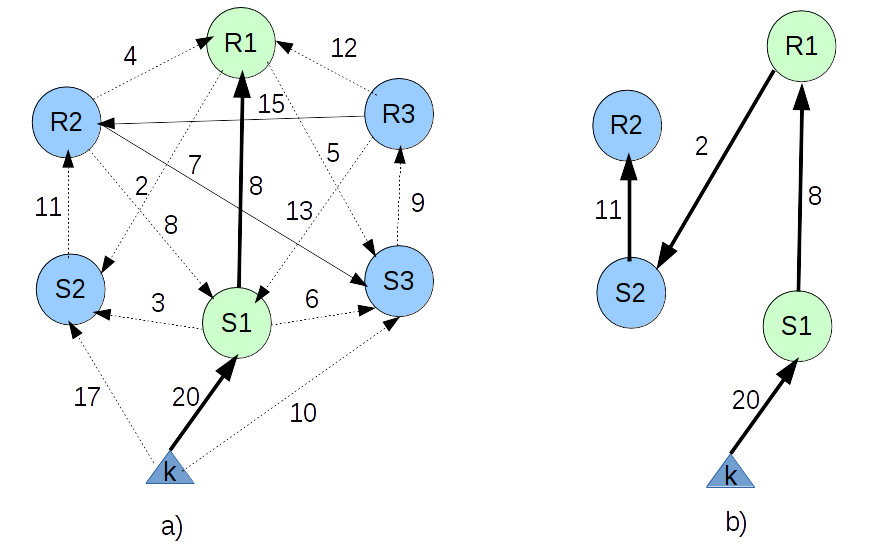
\includegraphics[width=1\linewidth]{images/pict1}}
	\caption{An example embodiment of a method of route constructing a single step}
	\label{ris:pict1}
\end{figure}

Fig. \ref {ris:pict1} represented by a weighted graph, which shows the example of the execution of one step of designing routes: \\
a) the original graph, which shows options to add new requests to the route; \\
b) the route, which was built by the construction method after first step.

\textit {Example.} Initially we have a request, which consists of a sender and receiver. The value of the cost function $\Omega $ are shown in the graph arcs (Figure \ref {ris:pict1}.). You need to add new requests to the route, using the criteria \ref{insert_kr} and \ref{kriterij}. The coefficient $\mu=0.5$.

		
\textit{Solution.}Consider the process of adding new requests. Of the two proposed requests $(\{S_2,R_2\},\{S_3,R_3\})$ it chooses the one which needs to be added firstly. Depending on the location where you can add application (beginning, end, middle), select the desired criteria. Thus, we find the optimal solution to insert a new order $\{S_2,R_2\}$:\\
$\min[c(k,S_1, \{S_2, R_2\}, R_1), c(k,\{S_2, R_2\}, S_1, R_1), c(k, S_1, R_1, \{S_2, R_2\})]=\min[3+11+4-0.5 \cdot 8; 17+11+8-0.5 \cdot 20; 2+11]=\min[14;26;13]$\\
We find the optimal place insert a new request $\{S_3,R_3\}$:\\ 
$\min[c(k,S_1, \{S_3, R_3\}, R_1), c(k,\{S_3, R_3\}, S_1, R_1), c(k, S_1, R_1, \{S_3, R_3\})]=\min[6+9+12-0.5 \cdot 8; 10+9+13-0.5 \cdot 20; 5+9]=\min[23;22;14]$.\\
From the solutions found will choose the solution with the lowest cost $c(k,v_i,u,v_{i+1})$.In this example, $c(k, S_1, R_1, \{S_2, R_2\}=13$.

Thus, the new route will consist of initial requests and new requests  $\{S_2,R_2\}$, which will be added to the end of the route.

			
\textit{Conclusion}: route in $\{S_1,R_1\}$ it is necessary to add  request $\{S_2,R_2\}$, which will be added to the end of the route


Fig. \ref{ris:pict2}presented the options of adding a new request to route $\{S_2,R_2\}$:\\
a) the option of adding request $\{S_2,R_2\}$ in the end of the route;\\
b) the option of adding request $\{S_2,R_2\}$ in the beginning of the route;\\
c) the option of adding request $\{S_2,R_2\}$ between nodes $\{S_1,R_1\}$.

Fig. \ref{ris:pict3} presented the options of adding a new request to route $\{S_3,R_3\}$:\\
a) the option of adding request $\{S_3,R_3\}$ in the end of the route;\\
b) the option of adding request $\{S_3,R_3\}$ in the beginning of the route;\\
c) the option of adding request $\{S_3,R_3\}$ between nodes $\{S_1,R_1\}$.

\begin{figure}[t]
	\center{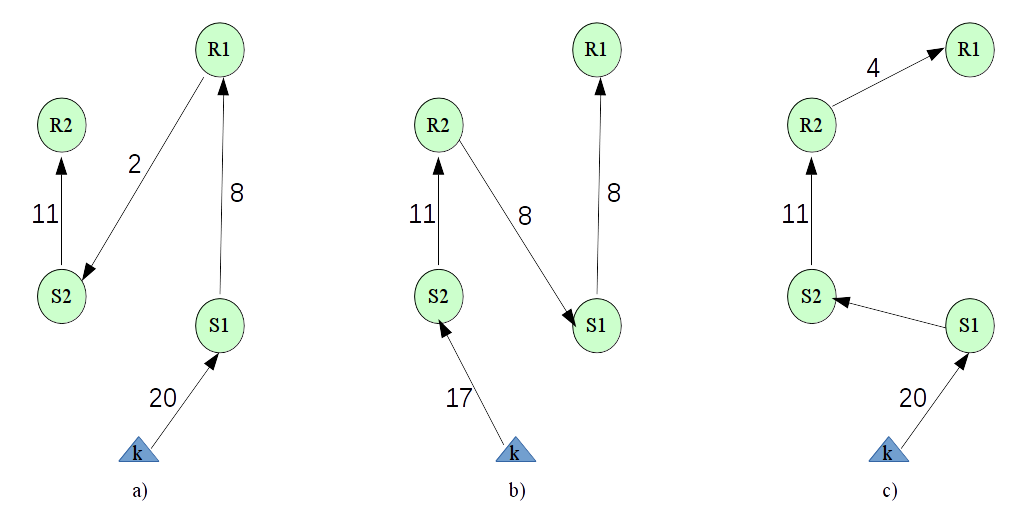
\includegraphics[width=1\linewidth]{images/pict2}}
	\caption{Options added  the request to route $\{S_2,R_2\}$}
	\label{ris:pict2}
\end{figure}

\begin{figure}[t]
	\center{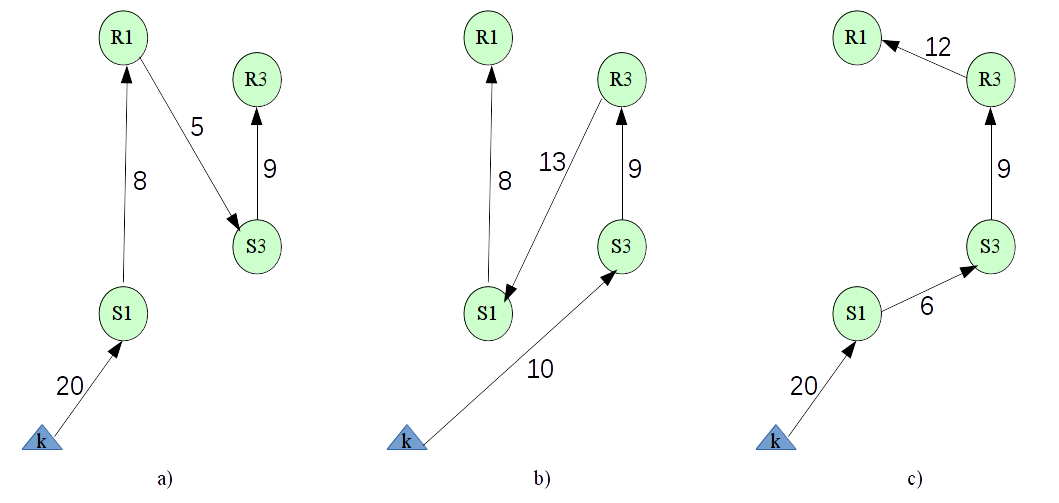
\includegraphics[width=1\linewidth]{images/pict3}}
	\caption{Options added the request to route $\{S_3,R_3\}$}
	\label{ris:pict3}
\end{figure}

\subsection{A Method of Forming Solutions Neighborhood}

During the work of the Tabu Search Algorithm should be carried out watching the neighborhood $N_{l}(\vec {u^i})$ current point $ \vec{u^i}$. In the calculation of the route in the neighborhood gets a sufficiently large number of points. But due to the limitations of our model features many of these points is not a solution to the problem. Therefore, due to the peculiarities of the considered discrete problem, we used the following method definition of a neighborhood.

Let $x^{k}(v)$ - node index $v$, $ v \in R \cup S $ in the path of the vehicle $ k \in C $. Each request consists of pairs $\{S, R \}$, where $S$ - sender, and $R$ - recipient. During the formation of the neighborhood, should be preserved the integrity of the route that is performed restrictions (\ref {main_cond_1} -- \ref {main_cond_4}). Above route requests $ Route_i $, $ i = 1, \dots n $ are performed permutation operation. The findings of the permutations of the vectors $ \vec {u} $ and is a neighborhood of $ N_{l} (\vec{u^i}) $. To swap transactions used movement and absorption.
	
Operation swallowing is shown in Figure \ref {ris: figures}. (A), which shows the two routes $Route_1 $ i $ Route_2 $. Route $ Route_1 $ consists of catch $ \{C_1, S_1, R_1, S_2, \\ R_2, S_3, R_3 \}$, and the route is $ Route_2 $ node $ \{C_2, S_4, R_4, S_5, R_5, S_6, R_6 \} $. During the operation of the absorption $ \{S_1, R_1 \} $ in the route $ Route_1 $, paste this application to route $ Route_2 $ can be performed on $ n + 1 $ positions.


\begin{figure}[h]
	\center{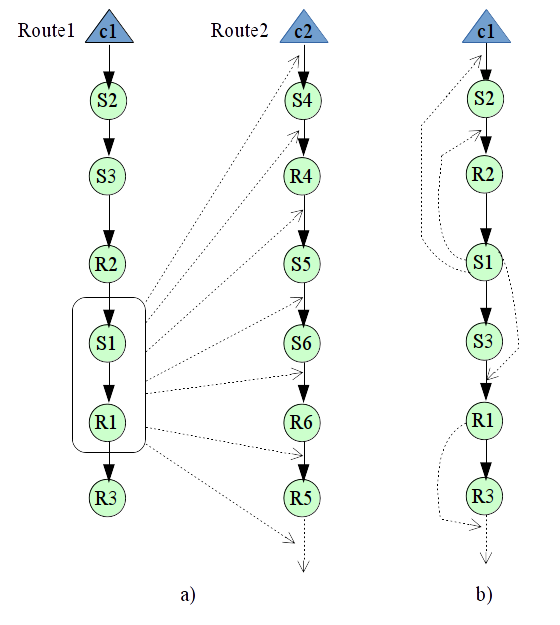
\includegraphics[width=0.75\linewidth]{images/neighboard.png}}
	\caption{Example of operations: a) absorption and b) moving}
	\label{ris:figures}
\end{figure}

The move operation is shown in figure \ref{ris: figures}. (B). This figure shows the route $ Route_1 $, which consists of nodes $ \{C_1, S_1, R_1, S_2, R_2, S_3, R_3 \} $. To save the route integrity: node $S_i $ (sender) can be visited only to $ R_i $ (recipient), on this basis during the move operation, the node $ S_i $ can move is to satisfy the condition $ 0 < x^{new} ( S_i) < \widetilde{u} (R_i) $, and  node $R_i$ can be moved until the condition is $ n^k \geq x^{new} (R_i)> \widetilde{u} (S_i) $.


\subsection{Analysis of the algorithm parameters}
The Tabu Search algorithm has two basic parameters: $h$ -- size of the list of prohibitions and $N_{neighbors}$ -- accepted count limit of size of neighbordhood $N_l(\vec{u})$. For the experiments, we constructed the test tasks on the basis of the capacity routing problems developed by Breedam, Fisher, Christofides and Eilon. To determine trends in time and cost of the decision we used exponential smoothing by a factor of $0.1$.

\begin{figure}[h]
	\hfil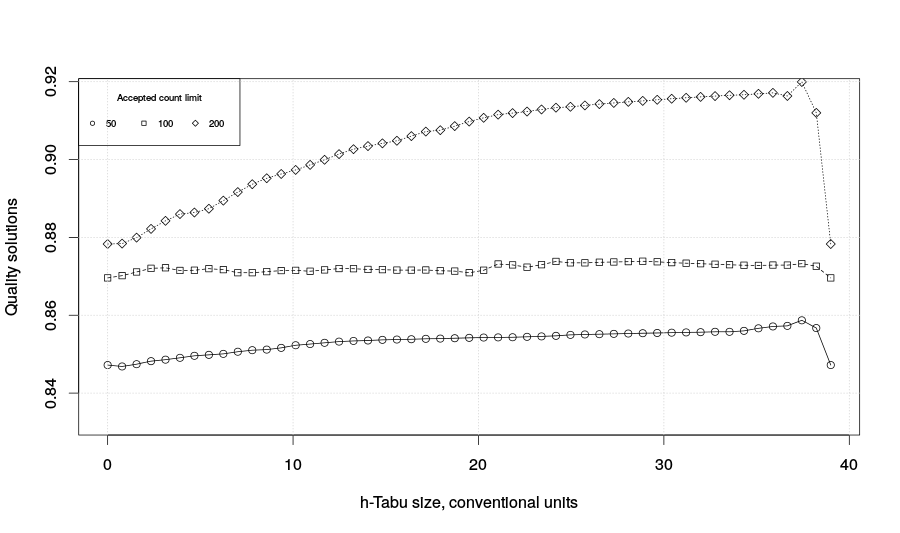
\includegraphics[height=3.0in]{images/tabuSize_stepCount}\hfil
	\caption
	{
	  The dependence of the quality of solutions on the size of the tabu list when using $ StepCount $ termination strategy
	}
	\label{aba:fig2}
\end{figure}

In this experiment we use two different breakpoint strategies: 
\begin{enumerate}
	\item $StepCount$ termination strategy --  terminates when an amount of steps has been reached;
	\item $TimeSpent$ termination strategy -- terminates when an amount of time has been reached.
\end{enumerate}

As should have been expected, for large values of the parameter a jam occurs in local optimum due to the large number of restrictions of movement in space. Otherwise if you select a too small tabu size, algorithm can still get stuck in a local optimum. In the first computational experiment we made finding the best solutions for different values of the tabu size parameter from interval $h \in [0, 40]$ (pict. \ref{aba:fig2} an pict. \ref{aba:fig3}).
\begin{figure}[h]
	\hfil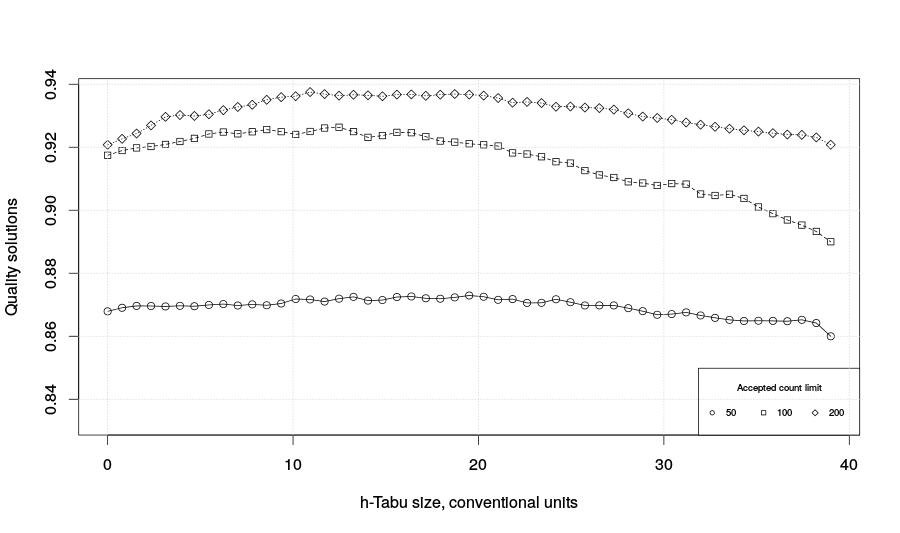
\includegraphics[height=2.2in]{images/tabuSize_time}\hfil
	\caption{
	  The dependence of the quality of solutions on the size of the tabu list when using $ TimeSpent $ termination strategy
	}
	\label{aba:fig3}
\end{figure}

\begin{figure}[h]
	\hfil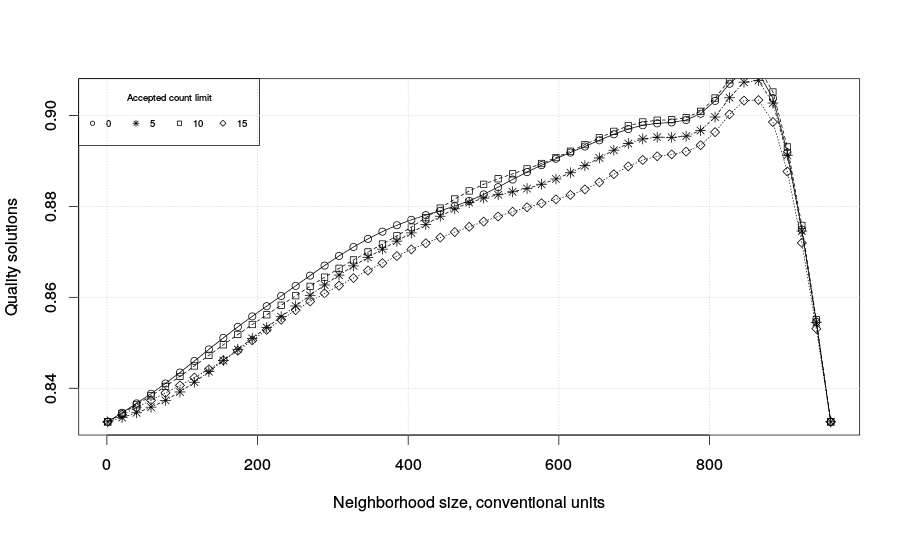
\includegraphics[height=2.2in]{images/acceptedCountLimit}\hfil
	\caption{
	  The dependence of the quality of solutions on the neighborhood size when using $ TimeSpent $ termination strategy
	}
	
	\label{aba:fig4}
\end{figure}

In the second experiment (see figure \ref{aba:fig4}) we built a relationship between the number $N_{neigh.}$ of viewed solutions neighborhood size $N_l(\vec{u})$ using $TimeSpent$ termination strategy. In this experiment we made finding the best solutions for different values of the neighborhood size parameter from interval $N_{neigh.}\in[750, 850]$.

\subsection{Modification}

The first generalized diagram is as follows. First, the set of solutions is constructed by route construction algorithm. Then every solution is improved by Tabu Search and choose the best solution according to the objective function.

Modification of the scheme is based on the hypothesis of ''On a large valley''\cite{opt_Kochetov}. According to this hypothesis, the average local optima are located much closer to the global than a randomly chosen point. There is a certain concentration of local optimum in a small part of the feasible region, which is figuratively called a large valley. If this assumption is true, then it is advisable to remember the best solutions and based on them design new original decision. We use this idea to solve the  Routing Courier Delivery Problem.

We proceed to the description of the algorithm in scheme \ref{alg:constructSolution}. Let $U^{opt}$ is a sorted array of optimal solutions by value of the objective function ascending,  ie:
\begin{equation} \label{u_sorted}
F(u^{opt}_1) \leq F(u^{opt}_2) \leq \ldots < F(u^{opt}_i) \leq \ldots \leq F(u^{opt}_{sizeof(U^{opt})})
\end{equation}
Each solution $u^{opt}_i$ gets into the population with a given probability $p^i_u$, the probability of selection decreases with increasing sequence number:
\begin{equation} \label{p_sorted}
p^1_u = 1 > p^2_u > \ldots > p^i_u> \ldots   > p^{sizeof(U^{opt})}_u,  p^{sizeof(U^{opt})}_u > 0
\end{equation}

\begin{algorithm}[H]

	\textbf{function constructSolution}( $U^{opt}, p_u, n^{min}_s$) \\
	// $U^{opt}$ -- a sorted set array of optimal solutions \\
	
	
	\If{$ sizeof(U^{opt}) <  n^{min}_s$}{
		// construct solution using heuristics(for example, Solomon alg.)\\
		$u^0 = heuristicsConscruction()$ \\
		\textbf{return} $u^0$
	}
	
	\While{$i < sizeof(U^{opt})$}{
		\If{$random(0.0,1.0) > p^i_u$}{
		   i = i + 1 \\
		   \textbf{goto} 8
		}
		$R_i = $randomly select a route from $u^{opt}_i$ solution;
		$u^0 = u^0 \cup R_i$
		i = i + 1\\
		
	}
	
	\If{$u^0 is not complete$}{
	   	$u^0 = heuristicsConscruction(u^0)$
	}
	
	\textbf{return} $u^0$
	
	\caption{Pseudo-code for heuristics construction algorithm.}
	\label{alg:constructSolution}
\end{algorithm}

It then crosses solutions by the following rule: with the first solution is randomly selected route $R_1$. Then another solution is selected from a route $R_2$ that does not include client requests from the first  route etc. If the client requests were not included in the solution $u^0$, then these requests are added by the construction heuristics algorithm (for example, Solomon algorithm).


Now we describe the primary function $SolveCDP()$ of the modified algorithm presented in pseudocode form in Scheme \ref{alg:modTabuSearch}. In this function using a loop is a sequential formation of an array of the best solutions $U^{opt}$ by means TabuSearch algorithm.   

Based on the results of the experiments described in the preceding section, we decided to set the parameters of the algorithm are not fixed values, but as a random variable of predetermined period. For example, the size of the tabu list $h$ is defined as the interval $[10,35]$(see pict. \ref{aba:fig2} and  pict. \ref{aba:fig3}) and the neighbordhood size $l=N_{neighbordhood}$ is defined as the interval $[6\cdot n,8.5\cdot n]$, where $n$ -- problem size (see pict. \ref{aba:fig4} ).

Let $\vec{\psi_i} = (\psi^1_i,\psi^2_i,\psi^3_i) = (\tilde{l_i},\tilde{p_i},\tilde{h_i})$ -- a set of values of the TabuSearch configuration parameters which was using for solving the problem in the step $i$.

Let $[\psi^j_{begin}, \psi^j_{end}]$ -- an optimal interval of the TabuSearch $j$ -parameter. For example: if $j=3$, then: $[\psi^3_{begin}, \psi^3_{end}]= [h_{begin}, h_{end}] = [10, 40] $. These intervals are initial data and they are set in the initialization block. 

The configuration parameters  $\psi^j_i $ are randomly selected from the interval $[\psi^j_{begin}, \psi^j_{end}]$ according to a distribution law. We proposed to build the distribution density $f_j(\psi^j_i)$ of the random variable $\psi^j_i$ as follows. At first, we define anchor points:
 
 \begin{equation} \label{anchor_points}
     \rho^j_i =  \dfrac{F(u^{opt}_1)}{avg[F(u^{opt}_k)]}, \forall k: \psi^j_k = \psi^j_i
 \end{equation}
 The number of anchor points $n_{\rho}$  is smaller than the set of optimal solutions, because a set of  anchor points are removed the same points $(n_{\rho} \leq  n_u)$.
 
The main idea is that the distribution density should be larger at those points (parameters $\psi^j_i$) in which high quality solutions than the points at which the low quality of solutions.
Therefore, we presented the distribution function $f_j(z)$ as a sum of kernel functions:
 \begin{equation} \label{dist_density}
 f_j(z) = \alpha_j * \sum\limits_{i=1}^{n_{\rho}}  \rho^j_i * K(z -  \psi^j_i)
 \end{equation}
 where: $K(x)$ -- kernel function, $ \alpha$ -- a normalizing parameter
 
 We have chosen as the kernel the function of parabolic type(known as an Epanechnikov function),  because during the experiments the best results were obtained using this function:
 \begin{equation} \label{dist_density}
  K(z) = 3/4 \cdot (1-z^2)
 \end{equation}
 

\begin{algorithm}[H]
	\textbf{function SolveCDP}( $n^{min}_s$) \\
	// Initialize variables:	\\
	
	$\psi = \emptyset$,
	$p_u = \emptyset$,
	$U^{opt} = \emptyset$,
	$i=0$ \\
	
	\While{the breakpoint is not triggered }{
		// set TabuSearch parameters \\
		\For{$j=1 \ldots 3$}{
	  	// $f_j$ -- the density distribution of the random \\
	  	// variable $\psi^j$ (TabuSearch parameter $l,p $ or $ h$) \\
	  	$\psi^j_i = random(\psi^j_{begin}, \psi^j_{end}, f_j) $
	  	}
	  	
		// Make solution using heuristics construction algorithms \\
		$u^0 = constructSolution(U^{opt} ,n^{min}_s)$ 
		
		// Improve solution $u^0$ using TabuSearch algorithm 
		$u^{opt}_i = TabuSearch(u^0, \vec{\psi_i})$ \\
		
		$U^{opt}  = U^{opt} \cup \{u^{opt}_i\}$ \\
		
		// Sort ascending optimums $U$ of the objective function \\
		$U^{opt} = sort(U^{opt})$\\
		$p^{i+1}_u = update(p^i_u)$\\
		
		i = i + 1\\
		
	}
	\textbf{return} $u^{opt}_1$
	
	\caption{Pseudo-code for modified tabu-search algorithm.}
	\label{alg:modTabuSearch}
\end{algorithm}

 The parameter $\alpha_j$ was introduced in the density function to perform the normalization condition:
 \begin{equation} \label{norm_cond}
 \int\limits_{\psi^j_{begin}}^{\psi^j_{end}} f_j(z)dz = 1  =>  (\alpha_j)^{-1} = \sum\limits_{i=1}^{n_{\rho}} \rho^j_i \cdot  \int\limits_{\psi^j_{begin}}^{\psi^j_{end}} K(z -  \psi^j_i) dz 
 \end{equation}

 The parameter $\alpha_j$ can be written in explicit form:
  \begin{equation} \label{norm_cond}
 \begin{split}
 (\alpha_j)^{-1} & = \dfrac{3}{4} \cdot \sum\limits_{i=1}^{n_{\rho}} \rho^j_i \cdot [(1 - (\psi^j_i)^2) \cdot (\psi^j_{end} - \psi^j_{begin}) + \\
 & + \psi^j_i \cdot ((\psi^j_{end})^2 - (\psi^j_{begin})^2) - 1/3 \cdot (\psi^j_{end})^3 - (\psi^j_{begin})^3)]
 \end{split}
 \end{equation}
 
 In figure \ref{aba:fig5} the results of an experiment in which  were presented a dependence of the quality of the solutions obtained by the classical and modified algorithms and  the breaking point time. As seen from the graph, with an increase in operating time of the computational scheme, the quality of solutions obtained using the modified algorithm is growing faster than using classical Tabu Search algorithm.
 
 \begin{figure}[h]
 	\hfil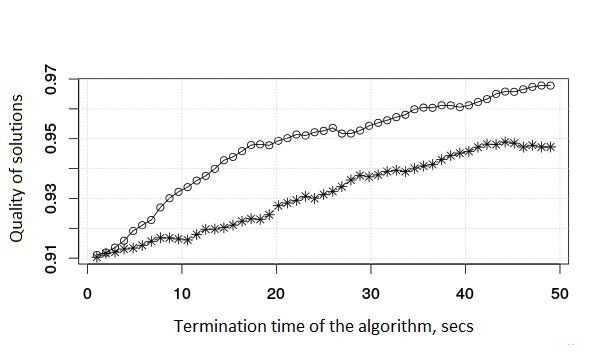
\includegraphics[height=3.0in]{images/tabu_mod.png}\hfil
 	\caption
 	{
 		The dependence of the quality of solutions and  the breaking point time by classic algorithm('$\times$' mark) with random selection tuning parameters and modified('o' mark) algorithms using $ TimeSpent $ termination strategy. 
 	}
 	\label{aba:fig5}
 \end{figure}
 
 
\subsection{Conclusion}
During the research has been investigated and implemented Tabu Search algorithm to solve the Routing Courier Delivery problem with time windows. Also a modified algorithm was developed  based on the Tabu Search Algorithm to improve the quality of solutions. Modified algorithm was given the best solutions in terms of the balance between the number of vehicles and the cost traveled.  In practice this algorithm can be used in intelligent systems for decision support, improving the quality of customer service and reducing waiting time, this will reduce fuel costs and depreciation of transport.
The analysis of the parameters of implemented algorithms allowed us to determine their optimal values for this class of routing problems. With the modified algorithm was found solutions of model problems, which in most cases have an acceptable deviation from the global optimum.

\begin{thebibliography}{99}
%In brackets we writes the name which is used for referencing.
\bibitem{RCDS} F.~Ordonez, Chen Wang, A New Approach for Routing Courier Delivery Services //METRANS Transportation Center:University of Southern California
Los Angeles,  2012, 81--115.

\bibitem{Delivery_Masson_2014} R.~Masson, F.~Lehued, O.~ Peton,The dial-a-ride problem with transfers. // Computers and Operations Research, Vol. 41, 2014, p. 12--23.
% http://www.sciencedirect.com/science/article/pii/S0191261599000168

\bibitem{Delivery_Babb_2005} T.~Babb, Pickup and Delivery Problem with Time Windows // Coordinated Transportation Systems: The State of the Art. Department of Computer Science University of Central Florida Orlando, Florida, 2005, 38 p.

\bibitem{vrp_shafeyev} R.~Shafeyev ,L.~Lyubchik, A some realization of Tabu Search algorithm for Solving the Transportation Problem with Time Constraints // Vestnik NTU "KhPI". – Kharkov: NTU
"KhPI", 2013. – No3 (977). – p. 35–39.

\bibitem{jlogistics}  R. Shafeyev. Java-based optimixation framework for solving routing problems.\\ url: http://jlogistics.net, 2015.

\bibitem{Delivery_Barnes_2000} W~Barnes, Solving the pickup and delivery problem with time windows using reactive tabu search // Transportation Research Part B: Methodological, Vol. 34 Issue 2, 2000, p. 107--121.

\bibitem{Delivery_Coltin_2014} B.~Coltin, M.~Veloso, Scheduling for Transfers in Pickup and Delivery Problems with Very Large Neighborhood Search // The Twenty-Eighth Conference on Artificial Intelligence, Quebec City, Canada, 2014, 7 p.
% http://www.cs.cmu.edu/~mmv/papers/14aaai-ColtinVeloso.pdf

\bibitem{opt_Goncharov} E.~Goncharov, Y~Kochetov, Probabilistic search with exclusions for discrete unconstrained optimization  //Discrete Analysis and Operations Research, Moscow, Serial 2. Vol. 9, 2002, p. 13-30.
%Гончаров Е.Н., Кочетов Ю.А. Вероятностный поиск с запретами для дискретных задач безусловной оптимизации // Дискрет. анализ и исслед. операций. Сер. 2. Т.9, № 2. 2002, с. 13-30.

\bibitem{opt_Kochetov}   Y~Kochetov, Probabilistic methods of local search for discrete optimization problems //Discrete Mathematics and Its Applications: Proceedings of youth lectures and scientific schools in discrete mathematics and its applications, Publishing House of the Center for Applied Research at the Mechanics and Mathematics. Faculty of Moscow State University, 2001, p. 84-117.  
%Кочетов Ю.А. Вероятностные методы локального поиска для задач дискретной оптимизации // Дискретная математика и ее приложения: Сб. лекций молодежных и научных школ по дискретной математике и ее приложениям. М.: Изд-во центра прикл. исслед. при мех-мат. фак. МГУ, 2001, с. 84-117; 

\bibitem{Tabu_search} O.~Braysy, M.~Gendreau, Vehicle Routing Problem with Time Windows, Part I: Route Constuction and local algorithms // Transportation science Vol.39 No. 1, 2005, p. 104-118.

\bibitem{Goldberg_Kennedy} V.~Goldberg, R.~Kennedy, An Efficient cost scaling algotirhm for the assignment problem, Math. Program., 1995, p. 153--177.  

\bibitem{problems_Christofides}  N. Christofides, S. Eilon, An algorithm for the vehicle dispatching problem //Operational Research Quarterly, 20, 1969, p. 309–318.

\bibitem{problems_Golden}  B. Golden, E. Wasil, J. Kelly, I-M. Chao. The impact of metaheuristics on solving the vehicle routing problem: Algorithms, problem sets, and computational results. In T. Crainic and G. Laporte, editors // Fleet Management and Logistics, Kluwer, Boston, 1998 p. 33–56.

\bibitem{problems_Taillard}  E. Taillard. VRP benchmarks.\\ url: http://mistic.heig-vd.ch/taillard/problemes.dir/vrp.dir/vrp.html, 1993.

\bibitem{Attanasio} A.~Attanasio, J.~Bregman,G.~Ghiani, E.~Manni. Real-time fleet management at Ecourier Ltd. Dynamic Fleet Management, volume 38 of Operations Research/Computer Science Interfaces, chapter 10, p.219--238, 2007.

\bibitem{Beaudry} A.~Beaudry, G.~Laporte, T.~Melo, Nickel. Dynamic transportation of patients in hospitals. Berichte des Fraunhofer ITWM, Nr. 104 :p.1--34, 2010.

\bibitem{Romero} M.Romero, L.Sheremetov and A.Soriano. A genetic algorithm for the pickup and delivery problem: An application to the helicopter offshore transportation. In Theoretical Advances and Applications of Fuzzy Logic and Soft Computing, volume 42 of Advances in Soft Computing, 2007, p. 35--44.

\bibitem{Kergosien} M.Romero, L.Sheremetov and A.Soriano. Yannick Kergosien, Christophe Lent, D. Piton, Jean-Charles Billaut. A tabu search heuristic for a dynamic transportation problem of patients between care units. 29 pages. 2010.

\bibitem{Sarak} H.~Sarak, A.~Satman. The degree-day method to estimate the residential heating natural gas consumption in Turkey: a case study. Pergamon, Energy 28 (2003) 929--939.




\end{thebibliography}



\end{document} \grid
\grid
\grid
